%!TEX root = ../dokumentation.tex

\chapter{Die Mathematik hinter Sudoku}

In diesem Kapitel sollen einige mathematische Fragen über Sudokus geklärt werden. Dazu gehören Fragen zur eindeutigen Lösbarkeit und wie diese bewiesen werden kann oder wie viele mögliche fertige Sudokus es denn überhaupt gibt. Zudem wird eine mathematische Beschreibung eines Sudokus gegeben und eine algorithmische Lösungsmethode, die ohne das Anwenden von Strategien, eine Lösung für ein Sudoku findet, falls es eine Lösung gibt.

\section{Abzählfragen}
In diesem Abschnitt soll geklärt werden wie viele mögliche Lösungen für ein vollständig ausgefülltes Sudokugitter existieren. Dabei werden zwei verschiedene Ansätze beschrieben. Besonders der Ansatz von Jarvis und Felgenhauer wird genauer angeschaut.

Ein trivialer Ansatz, um die Frage zu beantworten, wie viele vollständig ausgefüllten 9×9 Standard-Sudokus es gibt, könnte sein zeilenweise von links nach rechts oder spaltenweise von oben nach unten Zahlen einzutragen. Damit würden sich pro Zeile, Spalte oder Block $ 9! $ Möglichkeiten ergeben. Daraus ergeben sich
\begin{equation}\formelentry{Möglichkeiten vollständig ausgefüllte 9×9 Standard-Sudokus}
	(9!)^{9} = 1,1\cdot10^{50} 
\end{equation} 
Möglichkeiten, ein Sudokugitter auszufüllen. Von diesen ausgefüllten Gittern entsprechen aber nicht alle der Konvention, dass in den Zeilen, Reihen und Boxen jede Zahl von 1 bis 9 nur einmal vorkommen darf. 

Felgenhauer und Jarvis hatten für eine einzelne Unit dieselbe Herangehensweise. Anschließend haben Sie die möglichen Lösungen von drei linear verbundenen Blöcken errechnet, wie in Abbildung \ref{fig:SudokugitterTheorie} dargestellt. Für die Erklärungen werden im weiteren Verlauf exemplarisch die Blöcke I, II und III verwendet. 
\begin{figure}[H]
	\centering
	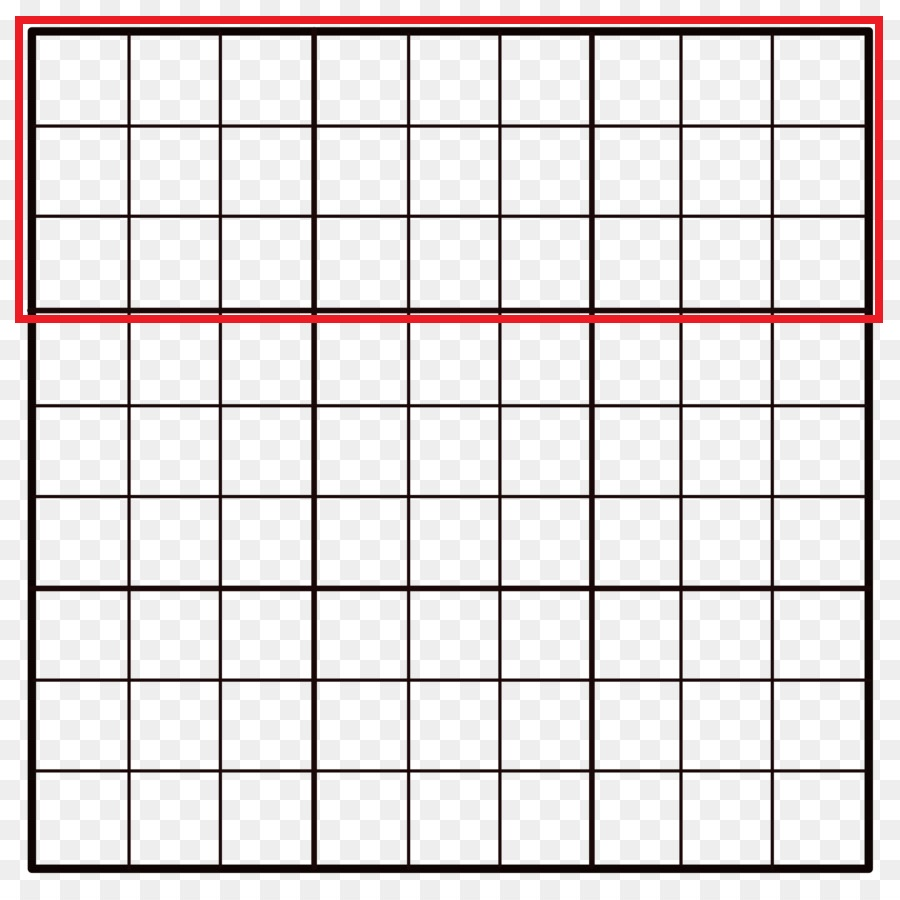
\includegraphics[width=0.3\textwidth]{images/SudokuTheorie.jpg}
	\caption{Markierung von drei linear verbundenen Blöcken}
	\label{fig:SudokugitterTheorie}
\end{figure}

Als Ausgangspunkt setzten Felgenhauer und Jarvis die Box I als ausgefüllt voraus. Zunächst berechnen sie die Anzahl von Möglichkeiten den Rest der obere Reihe mit zwei Sets aus jeweils drei Zahlen auszufüllen. So ein Dreier Set in das die Zahlen eingetragen werden sollen ist in Abbildung \ref{fig:SudokuDreierSet} markiert. Jedes Set aus drei Zahlen kann in $ 3! = 6 $ verschiedenen Anordnungen in die oberste Zeile eingetragen werden. Dabei müssen alle sechs Sets, die die Blöcke II und III formieren mit in Betracht gezogen werden. Dasselbe gilt für die Vertauschung der Anordnung der Sets der obersten Reihe. Dadurch ist der erste Teil $ 2 \cdot (3!)^{6} $ der folgenden Formel erklärt. 

Alle anderen 18 Möglichkeiten zwei dieser dreier Sets auszufüllen verhalten sich anders. Nachdem die obere Reihe in Block II und III ausgefüllt wurde, können Zahlen in den übrigen vier Sets aufgrund von fehlenden Einschränkungen vertauscht werden. Damit haben Felgenhauer und Jarvis für den zweiten Teil der Gleichung, $ 18 \cdot 3 \cdot (3!)^{6} $ argumentiert. Insgesamt gibt es also 56 Konfigurationen die sechs Dreier Sets weiter auszufüllen.
\begin{figure}[htbp]
	\centering
	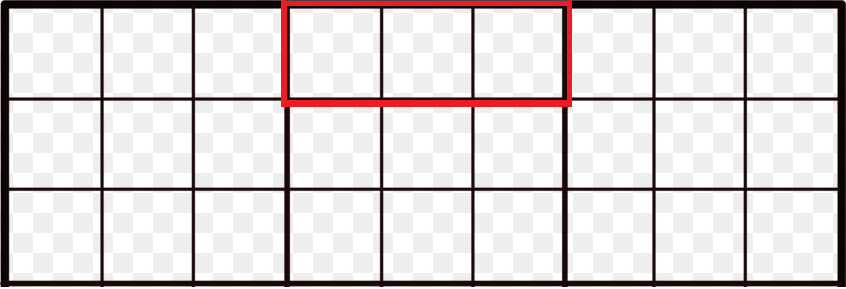
\includegraphics[width=0.3\textwidth]{images/SudokuDreierSet.png}
	\caption{Markierung eines Dreier Sets als Kombination aus Block und Zeile}
	\label{fig:SudokuDreierSet}
\end{figure}

Damit gibt es 
\begin{equation}
	\formelentry{Anzahl an Ergänzungen zu der ersten Reihe}
	2 \cdot (3!)^{6} + 18 \cdot 3 \cdot (3!)^{6} = 56 \cdot (3!)^{6} = 2612736
\end{equation} 
mögliche Erweiterungen einer bereits ausgefüllten Unit zu drei linear verbundenen Blöcken.  

Da es für eine vollständig ausgefüllte Unit aber $ 9! $ unterschiedliche Ausführungen gibt, muss man die die Möglichkeiten eine Unit auszufüllen mit den möglichen Ergänzungen multiplizieren.

Damit gibt es
\begin{equation}\formelentry{Anzahl an Möglichkeiten zu den obersten drei Reihen}
	9! \cdot 2612736 = 948109639680
\end{equation} 
Möglichkeiten, die oberen drei Reihen eines Sudokugitters auszufüllen.

Aus diesen 2612736 Möglichkeiten wollten Felgenhauer und Jarvis dann versuchen, die verbleibenden Blöcke des Sudokugitters mittels einer Brute-Force Methode auszufüllen. Da es mit den 2612736 Möglichkeiten immer noch ein zu großer Aufwand wäre, haben sich Felgenhauer und Jarvis drei Reduktionen überlegt, um die Anzahl an Möglichkeiten die ersten drei Reihen auszufüllen zu reduzieren.

Auf diese 2612736 Möglichkeiten haben Jarvis und Felgenhauer drei möglichen Reduktionen angewandt: die lexikographische Reduktion, die Reduktion der Permutationen und die Reduktion der Spalten. Durch diese Reduktionen werden Sudokus mit Lösungen, die sich durch Spiegeln, Drehen oder durch symmetrische Eigenschaften doppeln lassen, herausgefiltert. Aus Praktikabilitätsgründen kann in dieser Arbeit keine umfassende Übersicht der Reduktionen gegeben werden.

Nach den Reduktionen bleiben 44 Möglichkeiten, die Zeilen zwei und drei auszufüllen. Danach muss herausgefunden werden, wie viele Konfigurationen eines Sudokus es gibt, das Gitter zu vervollständigen. 

Felgenhauer und Jarvis haben in ihrer Veröffentlichung von 2006 die These aufgestellt, dass es 6.670.903.752.021.072.936.960, also ca. 6,7 Trilliarden  verschiedene, vollständig ausgefüllte Standard-Sudokus Rätsel gibt. Nach der Reduktion von symmetrischen Lösungen bleiben nur noch 5.5 Milliarden Lösungen. \cite{FelgenhauerJarvis} \cite[90\psqq]{althofer2014spiele}

\section{Komplexität}
Das folgende Unterkapitel gibt eine mathematische Definition eines Sudoku. Dabei wird eine allgemeine Beschreibung gegeben, die auf Sudokus die ein Problem n-ter Ordnung sind, angewendet werden kann.

Bei Sudokus, die in den Medien veröffentlicht werden, und immer eindeutig lösbar sein müssen, kann durch logische Schlussfolgerung das Sudokurätsel gelöst werden. Durch die eindeutige Lösbarkeit ist es nicht notwendig Fallunterscheidungen zu treffen, also auszuprobieren.

Mathematisch gesehen ist ein Sudoku ein Problem n-ter Ordnung. Dabei ist n eine natürliche Zahl. Auf einem $N\cdot N$ Gitter, wobei $N=n^2$ gilt, sind die Zahlen $1$ bis $N$ in das Gitter einzufügen. Dabei soll in jeder $1\cdot n$ Zeile, $n\cdot 1$ Spalte und $n\cdot n$ Block, jede der Zahlen $1$ bis $N$ genau einmal vorkommen. $N^2$ Felder des Gitters können dabei vorbelegt sein. Ein $9\cdot9$ Sudoku ist damit ein Problem 3-ter Ordnung. \cite{HerzbergMurty} 

\section{Eindeutige Lösbarkeit}\label{eindeutigLösbar}
Eine wichtige Eigenschaft von Sudokurätseln ist die eindeutige Lösbarkeit. In diesem Abschnitt wird erklärt was genau unter eindeutiger Lösbarkeit gemeint ist und wie viele Ziffern vorgegeben sein müssen um das zu erreichen.

Für ein Sudokugitter ohne vorgegebene Ziffern gibt es 5.472.730.538 (5,5 Milliarden) unterschiedliche, richtige Lösungen. Auch wenn nur eine oder zwei Ziffern vorgegeben werden, gibt es immer noch eine sehr große Anzahl an Lösungen für dieses Sudoku. 

Sudokus, die in irgendeiner Form veröffentlicht werden, sind normalerweise mit der Vorgabe einer eindeutigen Lösung erstellt. Sobald ein Sudoku nur eine korrekte Vervollständigung hat, ist es eindeutig lösbar. Daraus lässt sich folgern, dass in eindeutigen Sudokus in jede freie Zelle nur eine einzige Ziffer eingetragen werden kann, ohne die Regeln zu brechen.

Als notwendiges Kriterium für ein eindeutig lösbares Sudoku, müssen unter den vorgegebenen Zahlen mindestens acht unterschiedliche Zahlen von 1 bis 9 vorkommen. Dieses Kriterium ist gegeben durch den Fakt, dass bei nur sieben vorgegebenen unterschiedlichen Ziffern die beiden übrigen in der zugehörigen Lösung vertauscht werden können. \cite{HerzbergMurty} \cite[95\psqq]{althofer2014spiele}

\subsection{Anzahl vorgegebene Ziffern für ein eindeutiges Sudoku}  
Es gibt die Vermutung, dass die minimale Anzahl an vorgegebenen Ziffern 17 ist. Mittels Brute-Force Methoden wurden eindeutige Sudokus mit nur 17 vorgegebenen Zahlen gesucht. Daran wurde 2011 von einem Forschungsteam von Gary McGuire geforscht. Es gibt jedoch noch keinen mathematischen Beweis für die Vermutung. Diese Vermutung basiert also hauptsächlich auf dem Generieren und Ausprobieren von vielen unterschiedlichen Sudokurätseln mit nur 17 Ziffern und einer eindeutigen Lösung. \cite{FAZ} \cite[95\psqq]{althofer2014spiele}

\section{Algorithmische Lösungsmethode: Backtracking}
Um die eindeutige Lösbarkeit beweisen zu können muss ein Sudokurätsel gelöst werden. In der Studienarbeit wird das Überprüfen der eindeutigen Lösbarkeit mittels der algorithmischen Lösungsmethode des Backtracking bewiesen. Dieser Algorithmus wird im Verlaufe des Abschnitts erklärt und wie damit der Beweis der eindeutigen Lösbarkeit umgesetzt werden kann.

Backtracking ist eine Problemlösungsstrategie und mit der Rekursion verwandt. Es werden alle möglichen Lösungen ausprobiert und in jedem Schritt nach einer Abbruchbedingung überprüft. Die Bedingungen an das Problem, dass mit Backtracking gelöst werden sollen sind die Folgenden: 
\begin{enumerate}
	\item Ein Problem kann in endlich viele Teilschritte aufgeteilt werden
	\item Ein Teilschritt besitzt eine Abbruchbedingung
	\item Ein Teilschritt hat endlich viele Lösungsmöglichkeiten
\end{enumerate}

Für jedes Element des Problems, in diesem Fall für jede freie Zelle, werden alle möglichen Zustände ausprobiert. Die Zustände sind im Fall des Sudokus die Zahlen von eins bis neun. Wenn ein Zustand zulässig ist, also in der Zeile, Reihe oder Box die Zahl nicht bereits eingetragen ist, so wird rekursiv überprüft, ob es für den aktuellen Zustand eine Lösung gibt. Wenn es diese nicht gibt, wird der vorherige Schritt rückgängig gemacht und eine neue Lösung gesucht. 
Damit basiert Backtracking auf dem Trial-and-Error Prinzip und versucht eine erreichte Teillösung in eine Gesamtlösung zu transferieren. 

Bei $z$ möglichen Verzweigungen jeder Teillösung und einem möglichen Verzweigungsbaum mit der Tiefe von $N$ hat das Backtracking, sofern $z > 1$ ist im schlechtesten Fall mit $O(z^{N})$  eine exponentielle Laufzeit.
\begin{equation}\formelentry{Zeitkomplexität}
	1 + z + z^{2} + z^{3} + ... + z^{N} 
\end{equation} 

Wenn mittels des Backtrackings keine Lösung für das Sudoku gefunden wurde, gibt es keine Lösung. Wenn jedoch eine Lösung gefunden wurde, so ist noch nicht bewiesen, dass diese Lösung eindeutig ist. Um eine eindeutige Lösbarkeit zu garantieren, wird mittels Backtracking überprüft, dass keine weitere Lösung existiert.

Da es für das Lösen eines Sudokus keinen effizienteren Algorithmus gibt und bereits vor der Anwendung der Lösungsstrategie überprüft werden soll, ob es eine eindeutige Lösbarkeit gibt, ist dieser Ansatz am sinnvollsten. \cite[209\psqq]{logofatu2014grundlegende} \cite{knott_2017}

\subsection{Backtracking mit Brute-Force-Methode}
Backtracking mit der Brute-Force Methode funktioniert wie oben beschrieben auf dem Prinzip des Backtracking mit dem Ausprobieren aller möglichen Fällen. Mit dem ersten freien Feld probiert man mit der 1 beginnend, ob man zu einer Lösung kommt. Als Abbruchbedingung ist das nicht singuläre Auftreten der neu eingefügten Zahl in Reihe, Zeile und Box implementiert. 

Bei der Brute-Force Methode wird für jede freie Zelle von 1 bis 9 überprüft, ob diese Zahl in die Zelle eingetragen werden darf. Sobald eine Zahl eingetragen werden darf, wird das gemacht und mit der nächsten freien Zelle fortgefahren. Falls in einer Zelle die Abbruchbedingung für jede Zahl ausgelöst wurde, also keine Zahl mehr in die Zelle eingetragen werden kann, wird bei der vorherigen Zelle weiter versucht. Bis das Sudoku entweder vollständig gelöst ist, oder es keine Möglichkeiten mehr gibt und das Sudoku damit nicht lösbar ist.

Die Laufzeit des Algorithmus hängt von der Anzahl der freien Zellen ab und damit auch von der Anzahl der vorgegebenen Zahlen. Wenn viele Zahlen vorgegeben sind, dann ist die Tiefe $N$ des Verzweigungsbaums und damit auch die Laufzeit geringer. 


\lstset{
	frame=single,
	keywordstyle=\color{blue},
	commentstyle=\color{green},
	numbers=left,
}

\begin{lstlisting}[language=Python, caption={Funktion zum Lösen des Sudokurätsel}, label={lst:solve}]
	def solve(self, numbers=(1, SIZE + 1), board=None):
		"""
		Solves the SudokuBoard recursively via backtracking
		:return: False if not solvable, True if solved
		"""
		square = self.get_empty_square(board)
		
		if not square:
			return True
		
		for i in range(*numbers):
			if self.is_valid(i, square, board=board):
				board[square[0]][square[1]][0] = i
		
				if self.solve(numbers=numbers, board=board):
				return True
		
				board[square[0]][square[1]][0] = 0
		
		return False
\end{lstlisting}

\subsubsection{Abbruchbedingung}
Die Abbruchbedingung für das Backtracking ist mit einer eigenen Funktion \textit{is\_valid} umgesetzt.
\begin{lstlisting}[language=Python, caption={Abbruchbedingung durch Validierung der Lösungsvariante}, label={lst:valid}]
	def is_valid(self, number, position, board=None):
		...
		# Check row
		for j in range(SIZE):
			if board[position[0]][j][0] == number and j != position[1]:
			return False
		...
		# Check Box
		box_x = (position[1] // 3) * 3
		box_y = (position[0] // 3) * 3
		
		for i in range(box_y, box_y + 3):
			for j in range(box_x, box_x + 3):
				if board[i][j][0] == number and (i, j) != position:
				return False
		
	return True
\end{lstlisting}
Wie in dem Code implementiert, wird überprüftm, ob eine \textit{number} an einer bestimmten \textit{position} eingesetzt werden darf, oder ob diese Zahl bereits in der entsprechenden Reihe, Zeile oder Box vorhanden ist. Wenn die Zahl gültig ist, gibt die Funktion \textit{True} zurück, anderenfalls \textit{False}, womit die Abbruchbedingung als erfüllt gilt. \cite{knott_2017} 

\subsection{Beweis Eindeutigkeit}
Der Algorithmus des Backtrackings bricht nach dem Finden einer vollständigen Lösung für ein Sudoku ab. Damit ist bestätigt, dass es eine Lösung für das Sudoku Rätsel gibt, jedoch nicht, dass diese Lösung eindeutig ist. Um die Eindeutigkeit eines Sudokus zu beweisen, müsste nach dem Finden einer Lösung erfolglos versucht werden eine weitere Lösung zu finden.

Um die Eindeutigkeit eines Sudoku Rätsels zu beweisen, wird nach dem Finden einer Lösung das Backtracking nochmals von hinten begonnen. Damit ist gemeint, dass bei der ersten Lösungssuche in den freien Zellen die Zahlen von 1 bis 9 eingetragen werden und nach dem Abbruchkriterium überprüft wird. Beim Suchen nach einer zweiten Lösung beziehungsweise bei dem Beweis der Eindeutigkeit wird das Backtracking nochmals ausgeführt, dabei aber die Zahlen von 9 bis 1 in die freien Zellen eingetragen.

\begin{lstlisting}[language=Python, caption={Überprüfen ob ein Sudokurätsel eine eindeutige Lösung hat}, label={lst:uniquesolve}]
	def is_uniquely_solvable(self):
		temp_board = deepcopy(self.board)
		self.solve(numbers=(9, 0, -1), board=temp_board)
		return self.solved == temp_board
\end{lstlisting}

Nach dem Ausführen der beiden Backtracking Algorithmen werden die beiden gefundenen Lösungen miteinander verglichen. Wenn die dabei gefundenen Lösungen übereinstimmen, kann mit Garantie gesagt werden, dass das Sudoku eindeutig lösbar ist.

